%%

\section{Activity: build your FLOSS business model}

\begin{frame}
\frametitle{Description}
\begin{itemize}
  \item Think about an hypothetical start-up company.
  \item Activity based on or revolving around FLOSS.
  \item Create a short business model plan.
\end{itemize}
\end{frame}

\begin{frame}
\frametitle{Organization}

\begin{itemize}
 \item Groups of up to three persons (for discussing the plan)
\item Each student must make her own business project
 \item Name of project.
 \item Goals.
 \item Select license type and strategy.
 \item Briefly detail strategic areas.
\end{itemize}

\end{frame}

\begin{frame}
\frametitle{Economic aspects}

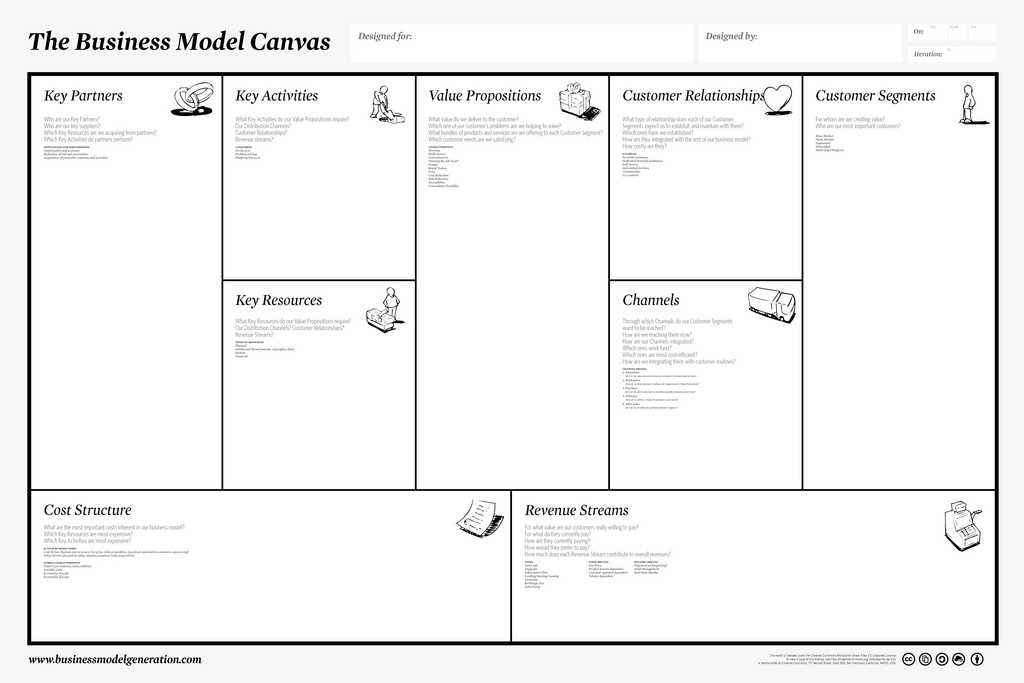
\includegraphics[width=10cm]{figs/business-model-canvas.jpg}

\end{frame}

\begin{frame}
\frametitle{Osterwalder's model}
Suggested order to fill in the canvas.
\begin{itemize}
 \item Clients segments
 \item Value proposal
 \item Channels
 \item Key resources
 \item Cost structure
 \item Revenues streams.
 \item Customer relationships
 \item Key activities
 \item Key partners
\end{itemize}

\end{frame}

\begin{frame}
 \frametitle{References}
\begin{itemize}
 \item \url{http://www.businessmodelalchemist.com/} 
 \item Business Model Generation: A Handbook for Visionaries, Game Changers, and Challengers, A. Osterwalder and Yves Pigneur. Wiley, July 2010.
 \item How to analyze an OSS business model (part 1 to 5).
  \begin{itemize}
   \item \url{http://carlodaffara.conecta.it/?p=372}
   \item \url{http://carlodaffara.conecta.it/?p=379}
   \item \url{http://carlodaffara.conecta.it/?p=387}
   \item \url{http://carlodaffara.conecta.it/?p=395}
   \item \url{http://carlodaffara.conecta.it/?p=413}
  \end{itemize}

\end{itemize}

  
 
 

\end{frame}

